% Author: Izaak Neutelings (June, 2018)
\documentclass[border=3pt,tikz]{standalone}
\usepackage{ifthen}
\usepackage{siunitx}
\usepackage{tikz}
\usetikzlibrary{hobby} % for ..
\usetikzlibrary{arrows.meta} % to control arrow size
\tikzset{>={Latex[length=4,width=4]}} % for LaTeX arrow head
\usetikzlibrary{calc,intersections,decorations.markings, positioning}
\usepackage{siunitx}
\usepackage{xcolor} % for colored text

\colorlet{mylightblue}{blue!20}
\colorlet{myblue}{blue!50!black}
\colorlet{mydarkblue}{blue!30!black}
\colorlet{mylightred}{red!10}
\colorlet{myred}{red!50!black}
\colorlet{mydarkred}{red!60!black}
\colorlet{mydarkgreen}{green!30!black}

%\tikzstyle{midarr}=[decoration={markings,mark=at position 0.5 with {\arrow{stealth}}},postaction={decorate}]
\tikzset{
  midarr/.style={decoration={markings,mark=at position #1 with {\arrow{stealth}}},postaction={decorate}},
  midarr/.default=0.5
}
\def\tick#1#2{\draw[thick] (#1) ++ (#2:0.03*\ymax) --++ (#2-180:0.06*\ymax)}


\begin{document}

% PHASE TRANSITIONS - ice -> water -> steam
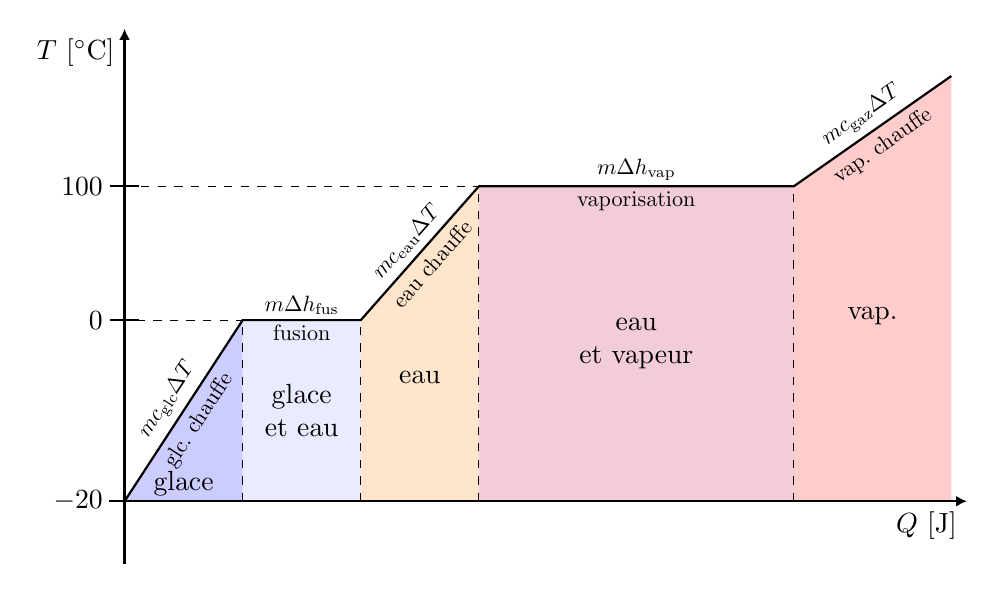
\begin{tikzpicture}
	\message{Phase transition of ice -> water -> steam^^J}
	\def\ymin{-0.8}
	\def\ymax{6}
	\def\xmin{-0.2}
	\def\xmax{10.6}
	\def\t{0.3}    % water/steam transition zone
	\def\ang{30.4} % angle gradient
	\coordinate (O) at (0.0,0.0);
	\coordinate (I) at (0.0,0.0); % ice
	\coordinate (M) at (1.5,2.3);  % melting
	\coordinate (W) at (3.0,2.3);  % water
	\coordinate (E) at (4.5,4.0);  % evaporate
	\coordinate (S) at (8.5,4.0);  % steam
	\coordinate (F) at (10.5,5.4);  % final
	\coordinate (Ex) at ($(E|-O)$); % x evaporation
	\coordinate (Ey) at ($(E-|O)$); % y evaporation
	\coordinate (Sx) at ($(S|-O)$); % x steam
	\coordinate (Fx) at ($(F|-O)$);

	% AREA
	\fill[mylightblue] (O) -- (M|-O) -- (M) -- cycle;
	\fill[blue!8] (M|-O) -- (M) -- (W) -- (W|-O) -- cycle;
	\fill[orange!20] (W) -- (W|-O) -- (Ex) -- (E) -- cycle;
	\fill[purple!20] (Ex) -- (E) -- (S) -- (Sx) -- cycle;
	\fill[red!20] (Sx) -- (S) -- (F) -- (Fx) -- cycle;
	% \begin{scope} % fade/gradient border
	% 	\clip (Ex) -- (Sx) -- (S) -- (E) -- cycle; % clip gradient rectangle
	% 	\draw[draw=none,transform canvas={rotate=\ang},top color=blue!8,bottom color=mylightred,shading angle=0]
	% 	({2.6*cos(\ang)},{-2.6*sin(\ang)-\t}) rectangle++(0.65*\xmax,\t); % diagonal border 
	% \end{scope}
	% \node[blue!40!black,left=4,below right=10pt] at (E) {eau};
	% \node[red!40!black,above left=10pt] at (Sx) {vapeur};

	% AXES
	\draw[->,thick] (0,\ymin) -- (0,\ymax) node[below left=0] {$T$ [\si{\degreeCelsius}]};
	\draw[->,thick] (\xmin,0) -- (\xmax+0.1,0) node[below left=0] {$Q$ [J]}; %[\si{J}]
	\draw[dashed] (W) -- (M-|O);
	\draw[dashed] (M|-O) -- (M);
	\draw[dashed] (W|-O) -- (W);
	\draw[dashed] (Ex) -- (E);
	\draw[dashed] (Ey) -- (S);
	\draw[dashed] (Sx) -- (S);
	\tick{I}{0} node[left=-1pt] {$-20$};
	\tick{M-|O}{0} node[left=-1pt] {$0$};
	\tick{Ey}{0} node[left=-1pt] {$100$};

	\draw[thick]
	(I) --
	coordinate (R1)
	(M)
	node[pos=0.5,above,scale=0.8,sloped, anchor=south] {$mc_{\rm glc}\Delta T$}
	node[pos=0.5,below,scale=0.8,sloped, anchor=north] {glc.\ chauffe}
	--
	coordinate (R2)
	(W)
	node[midway,above=-1pt,scale=0.8] {$m\Delta{h}_{\rm fus}$}
	node[midway,below=-1pt,scale=0.8] {fusion}
	--
	coordinate (R3)
	(E)
	node[pos=0.5,above,scale=0.8,sloped, anchor=south] {$mc_{\rm eau}\Delta T$}
	node[pos=0.5,below,scale=0.8,sloped, anchor=north] {eau chauffe}
	--
	coordinate (R4)
	(S)
	node[midway,above=-1pt,scale=0.8] {$m\Delta{h}_{\rm vap}$}
	node[midway,below=-1pt,scale=0.8] {vaporisation}
	--
	coordinate (R5)
	node[pos=0.5,above,scale=0.8,sloped, anchor=south] {$mc_{\rm gaz}\Delta T$}
	node[pos=0.5,below,scale=0.8,sloped, anchor=north] {vap.\ chauffe}
	(F);
	\node at ($(R1)!0.8!(R1|-O)$) {glace};
	\node[align=center] at ($(R2)!0.5!(R2|-O)$) {glace\\et eau};
	\node[align=center] at ($(R3)!0.5!(R3|-O)$) {eau};
	\node[align=center] at ($(R4)!0.5!(R4|-O)$) {eau\\et vapeur};
	\node[align=center] at ($(R5)!0.5!(R5|-O)$) {vap.};
\end{tikzpicture}


\end{document}
